\documentclass{scrreprt}
\usepackage{listings}
\usepackage{underscore}
\usepackage[bookmarks=true]{hyperref}
\usepackage[utf8]{inputenc}
\usepackage[english]{babel}
\usepackage{graphicx}
% \graphicspath{{work_packages/work_package_1/static/user-manual-images/}} % path relative to root
\graphicspath{{static/user-manual-images/}}
\hypersetup{
    pdftitle={Software Requirement Specification},    % title
    pdfauthor={Training Montage},                     % author
    pdfsubject={TeX and LaTeX},                        % subject of the document
    pdfkeywords={TeX, LaTeX, graphics, images}, % list of keywords
    colorlinks=true,       % false: boxed links; true: colored links
    linkcolor=blue,       % color of internal links
    citecolor=black,       % color of links to bibliography
    filecolor=black,        % color of file links
    urlcolor=purple,        % color of external links
    linktoc=page            % only page is linked
}

\def\myversion{0.1 }
\date{}

\usepackage{hyperref}
\begin{document}

\begin{flushright}
    \rule{16cm}{5pt}\vskip1cm
    \begin{bfseries}
        \Huge{SOFTWARE REQUIREMENTS\\ SPECIFICATION}\\
        \vspace{.9cm}
        for\\
        \vspace{.9cm}
        COE 1186 Project\\
        \vspace{.9cm}
        \LARGE{Version \myversion approved}\\
        \vspace{.9cm}
        Prepared by:\\
        Alec Rosenbaum\\
        Aric Hudson\\
        Isaac Goss\\
        Mitch Moran\\
        Parth Dadhania\\
        \vspace{1.9cm}
        Training Montage\\
        \vspace{.9cm}
        \today\\
    \end{bfseries}
\end{flushright}

\tableofcontents

\chapter{Module Name}

% picture(s) of overall gui
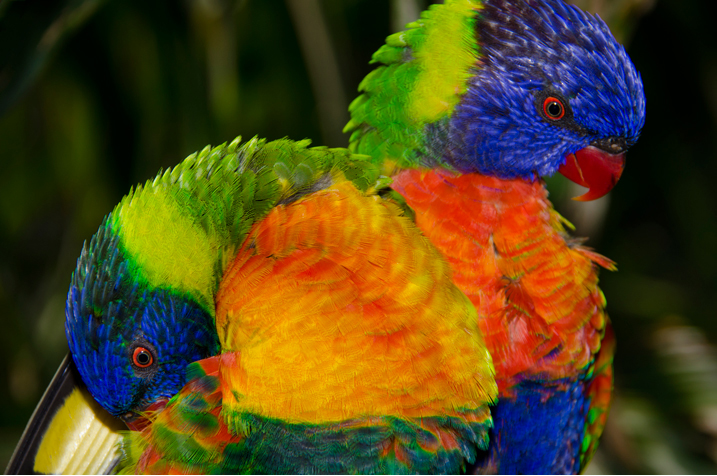
\includegraphics[width=\textwidth]{sample}

\section{GUI Section}

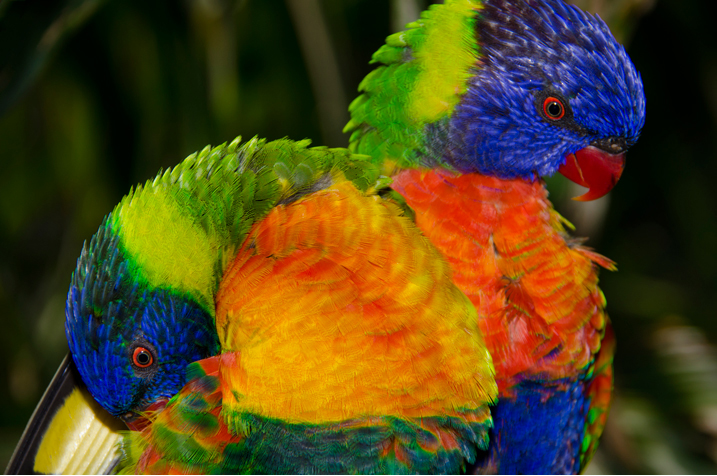
\includegraphics[trim={0 10cm 0 0},clip,width=\textwidth]{sample}
% trim={<left> <lower> <right> <upper>}

For example, show only the top of the original image for reference. asdf asdf asdf
asdf asdf asdf asdf asdf asdf asdf asdf.

There is this section that does this and that and has this stuff.

\section{GUI Section}
There will probably be a few GUI sections to elaborate on

\chapter{Track Model}

% picture(s) of overall gui
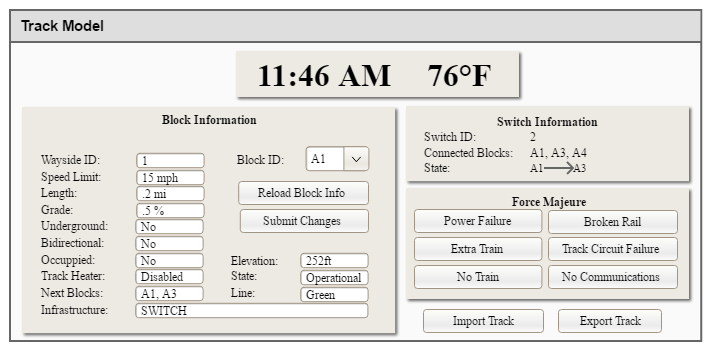
\includegraphics[width=\textwidth]{track-model}

\section{Block Information}

\begin{center}
    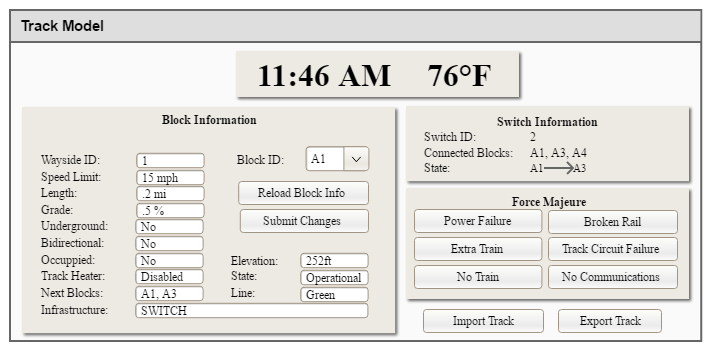
\includegraphics[trim={.5cm .5cm 11cm 3.6cm},clip,width=7.5cm]{track-model}
    % trim={<left> <lower> <right> <upper>}
\end{center}

The block information section allows the user to select a block (from a dropdown), view
stored block details, and reconfigure block defails. Once the user selects a block from the
dropdown, that blocks information will be populated onto the approprate fields. The user may
then reload the information about that block using the "Reload Block Info" button, or they
may edit any field and click the "Submit Changes" button to modify the details stored by
the Track Model.

The user may expect to see one or more of the follwing block states in the "State" field:
\begin{description}
    \item[Operational] The selected block is fully functional.
    \item[Broken Rail] The selected block includes a section of broken rail.
    \item[Extra Train] The selected block detects a train, when there is no train 
        actually present.
    \item[No Train] The selected block does not detect a train, when a train is present.
    \item[Power Failure] The selected block is experiencing a power failure.
    \item[No Communication] The selected block's communications aren't functional, thus no
        communication is relayed to any train present.
\end{description}

\section{Switch Information}

\begin{center}
    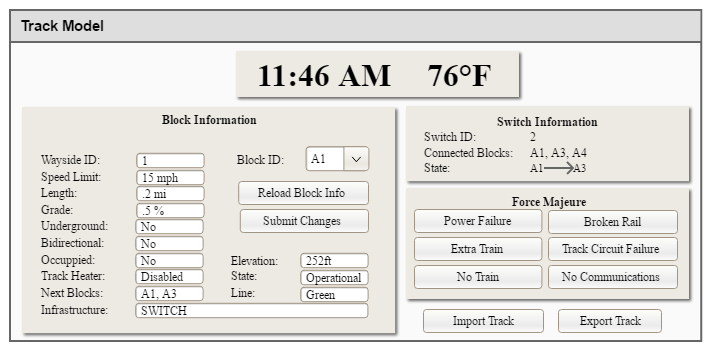
\includegraphics[trim={14.2cm 5.75cm .5cm 3.6cm},clip,width=6cm]{track-model}
    % trim={<left> <lower> <right> <upper>}
\end{center}

If there is a switch connected to the selected block, details will be presented in
thise section. Details include:
\begin{itemize}
    \item Switch ID
    \item Connected Blocks
    \item Switch State
\end{itemize}

\section{Force Majeure}

\begin{center}
    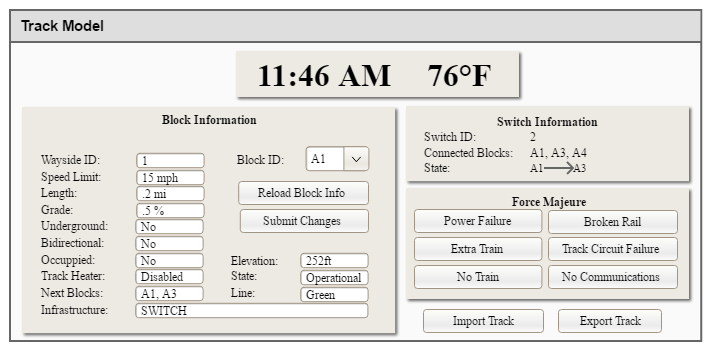
\includegraphics[trim={14.2cm 1.75cm .5cm 6.5cm},clip,width=7.5cm]{track-model}
    % trim={<left> <lower> <right> <upper>}
\end{center}

All options for causing Force Majeure failures are presented here. When the user clicks
an option, the Force Majeure failure is applied to the selected block.

\section{Track Import and Export}

\begin{center}
    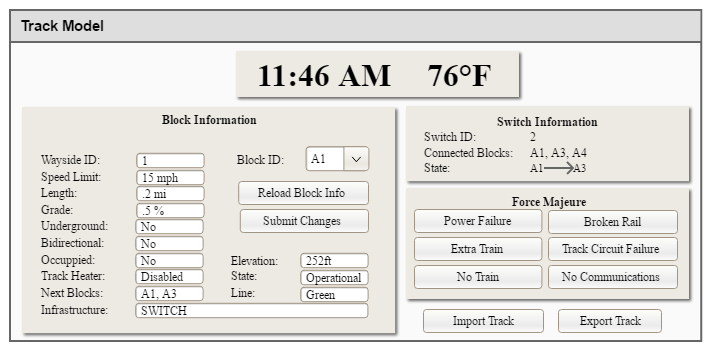
\includegraphics[trim={14.2cm .5cm .5cm 10.75cm},clip,width=7.5cm]{track-model}
    % trim={<left> <lower> <right> <upper>}
\end{center}

Track import and export options are presented here. The "Import Track" button allows
the entire track to be replaced with an imported track. The "Export Track" button allows
the entire track to be exported based on its current state.

\end{document}
